%% Glaukopis -- International Journal of Information Security (Springer) submission, v1.6-ijis (2026-10-24).
%% Port of doc/v1.6/glaukopis_v1.6.tex to Springer's svjour3 class in the journal's required
%% "twocolumn" format, numbered references (spmpsci.bst), single-blind (author-identified).
%% Build: bash build.sh   (pdflatex -> bibtex -> pdflatex x2); needs svjour3.cls, svglov3.clo, spmpsci.bst (in this folder).
%% Review model is single-blind (journal guidelines), so author names and affiliations stay in the manuscript.

\documentclass[border=3pt]{standalone}

\usepackage[T1]{fontenc}
\usepackage{amsmath,amssymb}
\usepackage{booktabs,array,tabularx,multirow}
\usepackage{graphicx}
\usepackage{xcolor}
\usepackage{xurl}
\usepackage{tikz}
\usetikzlibrary{arrows.meta,positioning,fit,backgrounds,calc}
\usepackage{pgfplots}
\usepgfplotslibrary{groupplots}
\pgfplotsset{compat=1.15}
\usepackage{listings}

\setlength{\emergencystretch}{2em}
\renewcommand{\topfraction}{0.95}
\renewcommand{\bottomfraction}{0.95}
\renewcommand{\textfraction}{0.03}
\renewcommand{\floatpagefraction}{0.75}
\setcounter{topnumber}{4}\setcounter{bottomnumber}{4}\setcounter{totalnumber}{8}\setcounter{dbltopnumber}{4}
\lstset{basicstyle=\footnotesize\ttfamily,breaklines=true,columns=fullflexible,keepspaces=true,frame=single,showstringspaces=false}
\newcommand{\code}[1]{\path{#1}}
\newsavebox{\fitbox}
\newcommand{\fitwidth}[1]{\sbox{\fitbox}{#1}\ifdim\wd\fitbox>\textwidth\resizebox{\textwidth}{!}{\usebox{\fitbox}}\else\usebox{\fitbox}\fi}
\newcommand{\ci}[2]{{\scriptsize[#1,\,#2]}}
\newcommand{\Abal}{A_{\mathrm{bal}}}
\newcommand{\Bbal}{B_{\mathrm{bal}}}
\newcommand{\Tbal}{T_{\mathrm{bal}}}
\definecolor{seriesblue}{HTML}{2A78D6}
\definecolor{refgray}{HTML}{52514E}


\begin{document}\setlength{\textwidth}{174mm}

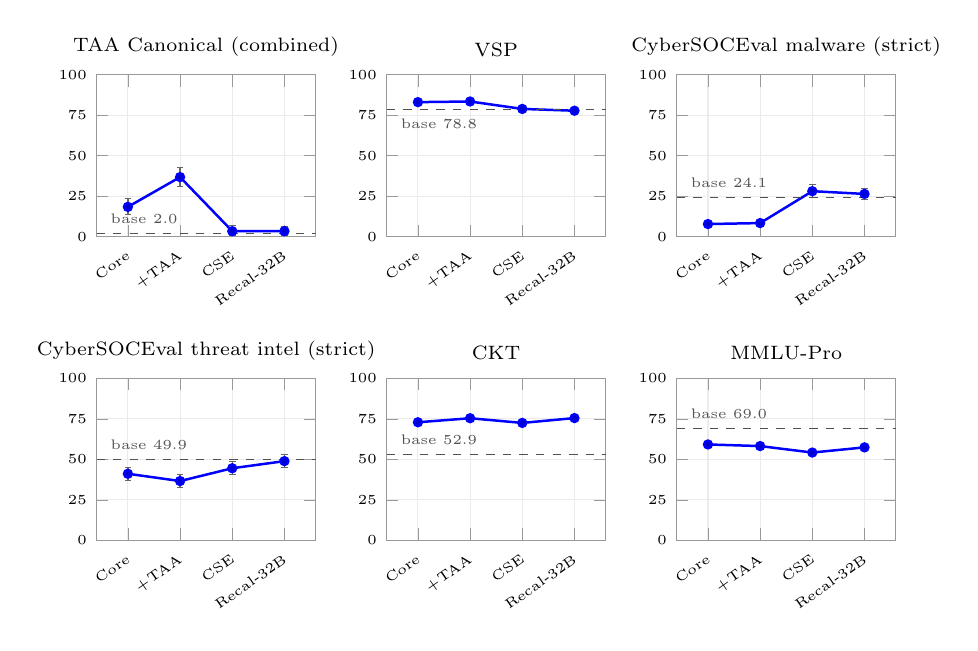
\begin{tikzpicture}
\begin{groupplot}[
  %% vertical sep must clear the rotated x tick labels of the upper row; at 13mm
  %% the lower row's titles printed on top of them.
  group style={group size=3 by 2, horizontal sep=9mm, vertical sep=18mm},
  width=0.36\textwidth, height=0.3\textwidth,
  ymin=0, ymax=100, ytick={0,25,50,75,100},
  xmin=-0.6, xmax=3.6, xtick={0,1,2,3}, xticklabels={Core,+TAA,CSE,Recal-32B}, x tick label style={font=\tiny, rotate=35, anchor=north east},
  y tick label style={font=\tiny}, title style={font=\scriptsize, yshift=-1mm},
  axis line style={black!40}, tick style={black!40}, grid=major, grid style={black!8},
  every axis plot/.append style={seriesblue, mark=*, mark size=1.4pt, line width=0.9pt, error bars/y dir=both, error bars/y explicit, error bars/error bar style={black!60, line width=0.5pt}, error bars/error mark options={black!60, rotate=90, mark size=1.2pt}}]
\nextgroupplot[title={TAA Canonical (combined)}]
\addplot coordinates {(0,18.4)+=(0,5.3)-=(0,4.9) (1,36.8)+=(0,5.7)-=(0,5.6) (2,3.4)+=(0,3.4)-=(0,2.6) (3,3.4)+=(0,3.0)-=(0,2.6)};
\draw[refgray, dashed] (axis cs:-0.6,2.0) -- (axis cs:3.6,2.0) node[pos=0.02, above right, font=\tiny, text=refgray] {base 2.0};
\nextgroupplot[title={VSP}]
\addplot coordinates {(0,83.1)+=(0,0.7)-=(0,0.7) (1,83.5)+=(0,0.6)-=(0,0.7) (2,78.9)+=(0,1.0)-=(0,1.0) (3,77.8)+=(0,1.1)-=(0,1.1)};
\draw[refgray, dashed] (axis cs:-0.6,78.8) -- (axis cs:3.6,78.8) node[pos=0.02, below right, font=\tiny, text=refgray] {base 78.8};
\nextgroupplot[title={CyberSOCEval malware (strict)}]
\addplot coordinates {(0,7.8)+=(0,2.3)-=(0,2.2) (1,8.4)+=(0,2.4)-=(0,2.2) (2,28.1)+=(0,4.1)-=(0,4.0) (3,26.4)+=(0,3.6)-=(0,3.5)};
\draw[refgray, dashed] (axis cs:-0.6,24.1) -- (axis cs:3.6,24.1) node[pos=0.02, above right, font=\tiny, text=refgray] {base 24.1};
\nextgroupplot[title={CyberSOCEval threat intel (strict)}]
\addplot coordinates {(0,41.1)+=(0,3.9)-=(0,4.0) (1,36.6)+=(0,3.8)-=(0,3.9) (2,44.5)+=(0,4.2)-=(0,4.1) (3,48.9)+=(0,4.1)-=(0,4.2)};
\draw[refgray, dashed] (axis cs:-0.6,49.9) -- (axis cs:3.6,49.9) node[pos=0.02, above right, font=\tiny, text=refgray] {base 49.9};
\nextgroupplot[title={CKT}]
\addplot coordinates {(0,72.9)+=(0,1.5)-=(0,1.6) (1,75.4)+=(0,1.6)-=(0,1.6) (2,72.5)+=(0,1.6)-=(0,1.6) (3,75.5)+=(0,1.6)-=(0,1.5)};
\draw[refgray, dashed] (axis cs:-0.6,52.9) -- (axis cs:3.6,52.9) node[pos=0.02, above right, font=\tiny, text=refgray] {base 52.9};
\nextgroupplot[title={MMLU-Pro}]
\addplot coordinates {(0,59.2)+=(0,0.9)-=(0,0.8) (1,58.2)+=(0,0.9)-=(0,0.9) (2,54.2)+=(0,0.9)-=(0,0.9) (3,57.4)+=(0,1.0)-=(0,0.9)};
\draw[refgray, dashed] (axis cs:-0.6,69.0) -- (axis cs:3.6,69.0) node[pos=0.02, above right, font=\tiny, text=refgray] {base 69.0};
\end{groupplot}
\end{tikzpicture}

\end{document}